\documentclass{standalone}
\usepackage{tikz}
\usetikzlibrary{shapes.geometric, arrows, positioning}

\begin{document} 
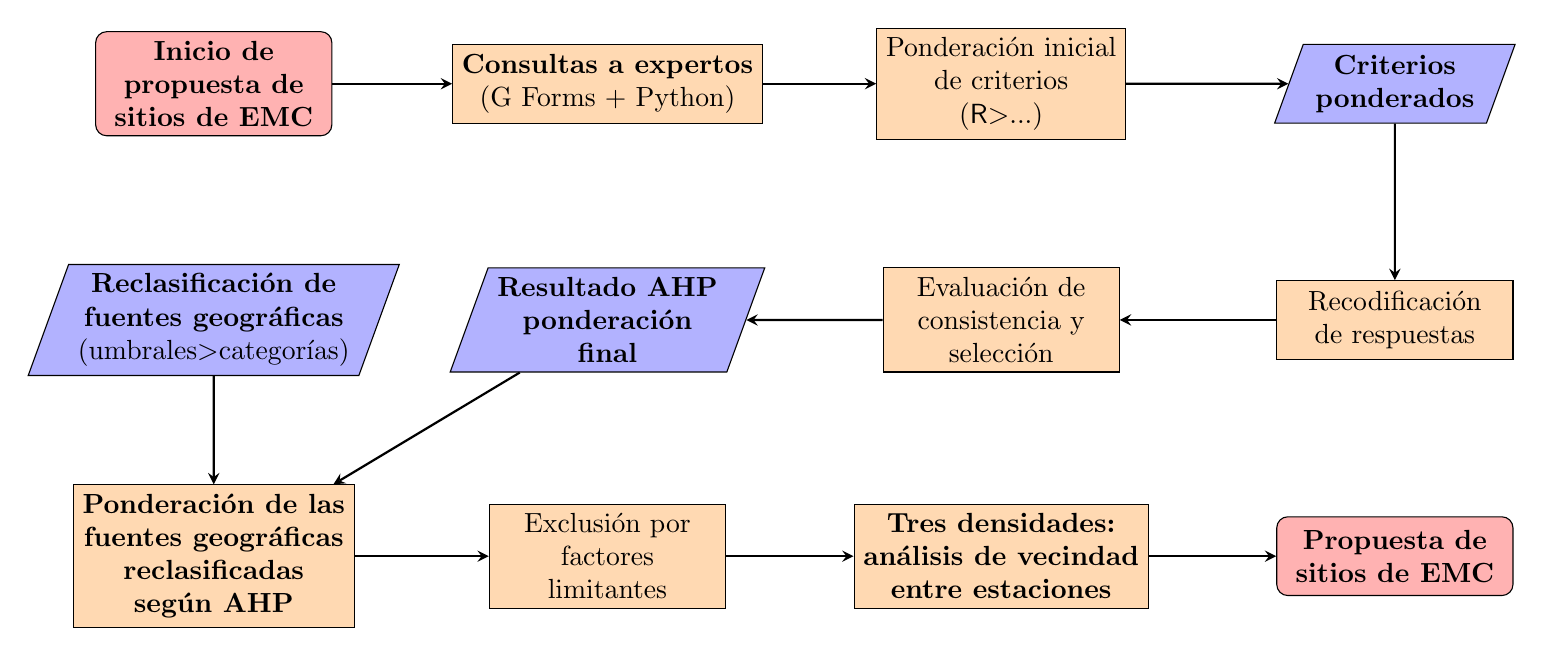
\begin{tikzpicture}[
  startstop/.style={rectangle, rounded corners, minimum width=3cm, minimum height=1cm,text centered, align=center, draw=black, fill=red!30},
  io/.style={trapezium, trapezium left angle=70, trapezium right angle=110, minimum width=3cm, minimum height=1cm, text centered, align=center, draw=black, fill=blue!30},
  process/.style={rectangle, minimum width=3cm, minimum height=1cm, text centered, align=center, draw=black, fill=orange!30},
  decision/.style={diamond, minimum width=3cm, minimum height=1cm, text centered, align=center, draw=black, fill=green!30},
  arrow/.style={thick,->,>=stealth}]

  % Nodes
  \node (start) [startstop] {\textbf{Inicio de} \\ \textbf{propuesta de} \\ \textbf{sitios de EMC}};
  \node (consultas) [process, right of=start, xshift=4cm] {\textbf{Consultas a expertos} \\ (G Forms + Python)};
  \node (ponderacion) [process, right of=consultas, xshift=4cm] {Ponderación inicial \\ de criterios \\ (\textsf{R}\textgreater...)};
  \node (criteriosponderados) [io, right of=ponderacion, xshift=4cm] {\textbf{Criterios} \\ \textbf{ponderados}};
  \node (recodificacion) [process, below of=criteriosponderados, yshift=-2cm] {Recodificación \\ de respuestas};
  \node (consistenciaseleccion) [process, left of=recodificacion, xshift=-4cm] {Evaluación de \\ consistencia y \\ selección};
  \node (resultadoahp) [io, left of=consistenciaseleccion, xshift=-4cm] {\textbf{Resultado AHP} \\ \textbf{ponderación} \\ \textbf{final}};
  
  \node (reclasificacionfuentesgeo) [io, left of=resultadoahp, xshift=-4cm] {\textbf{Reclasificación de} \\ \textbf{fuentes geográficas} \\ (umbrales\textgreater categorías)};

  \node (ponderacionfuentesgeo) [process, below of=reclasificacionfuentesgeo, yshift=-2cm] {\textbf{Ponderación de las} \\ \textbf{fuentes geográficas} \\ \textbf{reclasificadas} \\ \textbf{según AHP}};
  \node (exclusion) [process, right of=ponderacionfuentesgeo, xshift=4cm] {Exclusión por \\ factores \\ limitantes};
  \node (reajustedensidad) [process, right of=exclusion, xshift=4cm] {\textbf{Tres densidades:} \\ \textbf{análisis de vecindad} \\ \textbf{entre estaciones}};
  \node (end) [startstop, right of=reajustedensidad, xshift=4cm] {\textbf{Propuesta de} \\ \textbf{sitios  de EMC}};

  % Arrows
  \draw [arrow] (start) -- (consultas);
  \draw [arrow] (consultas) -- (ponderacion);
  \draw [arrow] (ponderacion) -- (criteriosponderados);

  \draw [arrow] (criteriosponderados) -- (recodificacion);
  \draw [arrow] (recodificacion) -- (consistenciaseleccion);
  \draw [arrow] (consistenciaseleccion) -- (resultadoahp);
  \draw [arrow] (resultadoahp) -- (ponderacionfuentesgeo);
  \draw [arrow] (reclasificacionfuentesgeo) -- (ponderacionfuentesgeo);  

  \draw [arrow] (ponderacionfuentesgeo) -- (exclusion);
  \draw [arrow] (exclusion) -- (reajustedensidad);
  \draw [arrow] (reajustedensidad) -- (end);
  
\end{tikzpicture}
\end{document}
